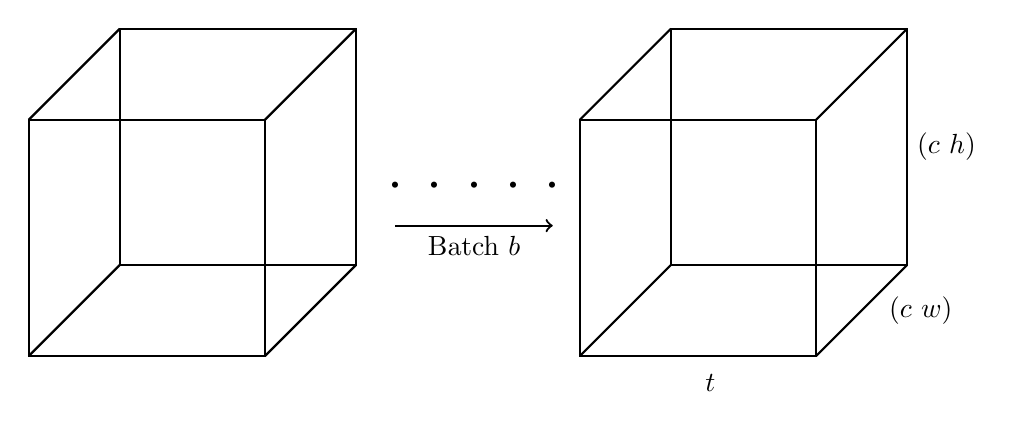
\begin{tikzpicture}
    % First cube
        % variables
        \def\cubeWidth{3}
        \def\cubeHeight{3}
        \def\cubeDepth{3}
    
        % Cube points
        \coordinate (A) at (0, 0, 0);
        \coordinate (B) at (\cubeWidth, 0, 0);
        \coordinate (C) at (\cubeWidth, \cubeHeight, 0);
        \coordinate (D) at (0, \cubeHeight, 0);
        \coordinate (E) at (0, 0, \cubeDepth);
        \coordinate (F) at (\cubeWidth, 0, \cubeDepth);
        \coordinate (G) at (\cubeWidth, \cubeHeight, \cubeDepth);
        \coordinate (H) at (0, \cubeHeight, \cubeDepth);
    
        % Draw cube
        \draw[thick] (A) -- (B) -- (C) -- (D) -- cycle;
        \draw[thick] (E) -- (F) -- (G) -- (H) -- cycle;
        \draw[thick] (A) -- (E);
        \draw[thick] (B) -- (F);
        \draw[thick] (C) -- (G);
        \draw[thick] (D) -- (H);
    
        % Axes
        \node at (0.5, -1.5, 0) {$t$};
        \node at (\cubeWidth + 0.5, \cubeHeight/2, 0) {$(c\ h)$};
        \node at (\cubeWidth + 0.75, 0, \cubeDepth/2) {$(c\ w)$};

    % Second cube
        % variables
        \def\cubeShiftX{-7}
        \def\cubeShiftY{0}
    
        % Cube points (shifted)
        \coordinate (A') at (\cubeShiftX, \cubeShiftY, 0);
        \coordinate (B') at (\cubeShiftX + \cubeWidth, \cubeShiftY, 0);
        \coordinate (C') at (\cubeShiftX + \cubeWidth, \cubeShiftY + \cubeHeight, 0);
        \coordinate (D') at (\cubeShiftX, \cubeShiftY + \cubeHeight, 0);
        \coordinate (E') at (\cubeShiftX, \cubeShiftY, \cubeDepth);
        \coordinate (F') at (\cubeShiftX + \cubeWidth, \cubeShiftY, \cubeDepth);
        \coordinate (G') at (\cubeShiftX + \cubeWidth, \cubeShiftY + \cubeHeight, \cubeDepth);
        \coordinate (H') at (\cubeShiftX, \cubeShiftY + \cubeHeight, \cubeDepth);
    
        % Draw the second cube
        \draw[thick] (A') -- (B') -- (C') -- (D') -- cycle;
        \draw[thick] (E') -- (F') -- (G') -- (H') -- cycle;
        \draw[thick] (A') -- (E');
        \draw[thick] (B') -- (F');
        \draw[thick] (C') -- (G');
        \draw[thick] (D') -- (H');

    % Three dots
        % variables
        \def\dotStartX{-3.5}
        \def\dotStartY{1}
        \def\dotShiftX{0.5}
        \def\dotShiftY{0}
    
        % dots
        \node at (\dotStartX, \dotStartY) {\huge$\cdot$};
        \node at (\dotStartX + \dotShiftX, \dotStartY + \dotShiftY) {\huge$\cdot$};
        \node at (\dotStartX + \dotShiftX * 2, \dotStartY + \dotShiftY * 2) {\huge$\cdot$};
        \node at (\dotStartX + \dotShiftX * 3, \dotStartY + \dotShiftY * 3) {\huge$\cdot$};
        \node at (\dotStartX + \dotShiftX * 4, \dotStartY + \dotShiftY * 4) {\huge$\cdot$};


    % Arrow
    \draw[->, thick] (-3.5, 0.5) -- (-1.5, 0.5) node[midway, below] {Batch $b$};
\end{tikzpicture}